% =============================================================================
% APPENDIX VVV.1: STRATEGY-ROADMAP: Technological Roadmap and Scenarios
% =============================================================================
% Module: EBF_VVV_STRATEGY_ROADMAP
% Version: 2.0 (January 2026)
% Status: Draft
% Language: English
%
% This appendix provides strategic analysis of technological evolution
% scenarios (2024-2030+) and their implications for EBF deployment.
% Covers AI capability trajectories, market dynamics, and platform strategies.
%
% Category: STRATEGY
% Core Question: What technological and market scenarios should guide
%                EBF deployment strategy over the next 5-7 years?
%
% =============================================================================

% =============================================================================
% CROSS-REFERENCE STRUCTURE
% =============================================================================
%
% CHAPTER LINKAGE (Required):
% - Primary Chapter: Chapter 15: Future Directions and Research Agenda
% - Secondary Chapters: Chapter 1 (Introduction), Chapter 14 (Implementation)
%
% This appendix provides foundation for strategic planning:
%
% DEPENDENCIES (what this appendix REQUIRES):
% - Appendix CTW (CORE-WHEN): Context framework ($\Psi$) for scenario analysis
% - Appendix EST (CORE-WHERE): Parameter estimation for calibration
% - Appendix LLM1 (METHOD-LLMMC): LLM Monte Carlo methods
%
% DEPENDENTS (what REQUIRES this appendix):
% - Appendix VVV.2: Product roadmap builds on scenario analysis
% - Appendix VVV.3: Partnership strategy depends on platform scenarios
%
% =============================================================================

\begin{tcolorbox}[colback=purple!5!white, colframe=purple!75!black,
    title=Chapter Linkage]

\textbf{Primary Chapter:} Chapter 15: Future Directions and Research Agenda
\begin{itemize}[nosep]
\item Section 15.1: Technology Evolution $\leftrightarrow$ This Appendix Section VVV.1.1
\item Section 15.3: Strategic Scenarios $\leftrightarrow$ This Appendix Section VVV.1.2
\end{itemize}

\textbf{Secondary Chapters:}
\begin{itemize}[nosep]
\item Chapter 1: Introduction --- references strategic positioning
\item Chapter 14: Implementation --- references technology dependencies
\end{itemize}

\textbf{Reading Guide:}
\begin{itemize}[nosep]
\item For conceptual overview: Read Chapter 15 first
\item For formal scenario analysis: This appendix provides complete specification
\item For technology details: See Appendix LLM1 (METHOD-LLMMC)
\end{itemize}

\end{tcolorbox}

%%%%%%%%%%%%%%%%%%%%%%%%%%%%%%%%%%%%%%%%%%%%%%%%%%%%%%%%%%%%%%%%%%%%%%%%%%%%%%%
\chapter{STRATEGY-ROADMAP: Technological Roadmap and Scenarios}
\label{app:vvv1-roadmap}
%%%%%%%%%%%%%%%%%%%%%%%%%%%%%%%%%%%%%%%%%%%%%%%%%%%%%%%%%%%%%%%%%%%%%%%%%%%%%%%

\begin{abstract}
This appendix analyzes technological evolution scenarios for EBF deployment
from 2024 to 2030+. We identify three axes of uncertainty (AI capability,
behavioral AI market maturity, platform landscape) and derive four archetypal
scenarios: Golden Window, Red Ocean, Slow Burn, and Platform Play. Each
scenario implies different strategic priorities for framework deployment,
partnership formation, and product development. The analysis connects to the
EBF context framework ($\Psi$) by treating technological and market conditions
as external context that shapes optimal strategy.
\end{abstract}

\begin{tcolorbox}[colback=blue!5!white, colframe=blue!75!black,
    title=Quick Reference: Technological Roadmap]
\textbf{Appendix:} VVV1-ROADMAP (STRATEGY)


\textbf{Core Question:} What technological and market scenarios should guide
EBF deployment strategy over the next 5-7 years?

\textbf{Key Framework:}
\begin{equation}
C^*_{strategy}(\Psi_{tech}, \Psi_{market}, \Psi_{platform}) = \arg\max E[Q | \text{Scenario}]
\end{equation}

\textbf{Key Concepts:}
\begin{itemize}[nosep]
\item Three Axes of Uncertainty: AI capability, market maturity, platform landscape
\item Four Scenarios: Golden Window (30-40\%), Red Ocean (25-35\%), Slow Burn (15-25\%), Platform Play (10-20\%)
\item GPT $\to$ Skills paradigm shift: Context detection enables automatic EBF invocation
\item Technology dependencies: Skills/MCP, multi-modal, structured output, agent orchestration
\end{itemize}

\textbf{Cross-References:} Appendix CTW (CORE-WHEN), Appendix EST (CORE-WHERE),
Appendix LLM1 (METHOD-LLMMC), Appendix VVV.2 (Product Roadmap)
\end{tcolorbox}

%%%%%%%%%%%%%%%%%%%%%%%%%%%%%%%%%%%%%%%%%%%%%%%%%%%%%%%%%%%%%%%%%%%%%%%%%%%%%%%
% -----------------------------------------------------------------------------
% APPENDIX SCOPE BOX
% -----------------------------------------------------------------------------

\begin{tcolorbox}[
    colback=orange!5!white,
    colframe=orange!75!black,
    title={\textbf{Appendix Scope: Ziel / In-Scope / Out-of-Scope / Constraints}},
    fonttitle=\bfseries
]

\textbf{Ziel (Objective):}
\begin{itemize}[nosep]
    \item Given uncertainty in AI capabilities, market development, and platform
dynamics, what strategic positioning maximizes EBF's expected impact and
sustainability over the 2024-2030+ timeframe?
\end{itemize}

\textbf{In-Scope:}
\begin{itemize}[nosep]
    \item The Fundamental Question
    \item Technological Roadmap: 2024--2030+
    \item The Four Scenarios
    \item Key Results
    \item Worked Example
\end{itemize}

\textbf{Out-of-Scope (delegiert an andere Appendices):}
\begin{itemize}[nosep]
    \item CORE-WHEN $\rightarrow$ Appendix CTW
    \item CORE-WHERE $\rightarrow$ Appendix EST
    \item CORE-WHEN $\rightarrow$ Appendix CTW
    \item CORE-WHERE $\rightarrow$ Appendix EST
    \item CORE-WHEN $\rightarrow$ Appendix CTW
\end{itemize}

\textbf{Constraints (Anwendungsgrenzen):}
\begin{itemize}[nosep]
    \item [TODO: Define when this appendix does NOT apply]
    \item [TODO: Define required prerequisites]
    \item [TODO: Define known limitations]
\end{itemize}

\textbf{Lieferobjekte (Deliverables):}
\begin{itemize}[nosep]
    \item 5 Table(s)
    \item 2 Equation(s)
    \item Worked Example(s)
\end{itemize}

\end{tcolorbox}


\section{The Fundamental Question}
\label{sec:vvv1-fundamental}
%%%%%%%%%%%%%%%%%%%%%%%%%%%%%%%%%%%%%%%%%%%%%%%%%%%%%%%%%%%%%%%%%%%%%%%%%%%%%%%

\subsection{Why This Matters}

The EBF framework exists at the intersection of behavioral science and
artificial intelligence. Its deployment success depends critically on
how both domains evolve. Understanding potential technology trajectories
enables:
\begin{itemize}
    \item \textbf{Resource allocation:} Prioritizing development efforts
    \item \textbf{Partnership timing:} When to engage with platforms
    \item \textbf{Risk management:} Preparing for adverse scenarios
    \item \textbf{Opportunity capture:} Recognizing and acting on favorable windows
\end{itemize}

\subsection{The Core Problem}

Technology evolution is inherently uncertain, yet strategic decisions must
be made today. The challenge is developing a scenario framework that:
\begin{enumerate}
    \item Captures the key dimensions of uncertainty
    \item Identifies meaningful scenario archetypes
    \item Maps scenarios to strategic responses
    \item Provides trigger events for scenario monitoring
\end{enumerate}

\begin{tcolorbox}[colback=red!5!white, colframe=red!75!black,
    title=The Fundamental Question]
\textbf{Given uncertainty in AI capabilities, market development, and platform
dynamics, what strategic positioning maximizes EBF's expected impact and
sustainability over the 2024-2030+ timeframe?}
\end{tcolorbox}


%%%%%%%%%%%%%%%%%%%%%%%%%%%%%%%%%%%%%%%%%%%%%%%%%%%%%%%%%%%%%%%%%%%%%%%%%%%%%%%
\section{Technological Roadmap: 2024--2030+}
\label{sec:vvv1-roadmap-detail}
%%%%%%%%%%%%%%%%%%%%%%%%%%%%%%%%%%%%%%%%%%%%%%%%%%%%%%%%%%%%%%%%%%%%%%%%%%%%%%%

\subsection{The Three Axes of Uncertainty}

The future of AI and behavioral technology depends on three independent dimensions:

\begin{tcolorbox}[colback=blue!5!white, colframe=blue!75!black,
    title=Three Axes of Technological Uncertainty]

\textbf{Axis 1: AI Capability Evolution}
\begin{itemize}[nosep]
\item \textbf{Conservative}: Incremental LLM improvements, current architecture
\item \textbf{Moderate}: Significant agent capabilities, multi-modal, reasoning
\item \textbf{Aggressive}: AGI-adjacent capabilities, autonomous agents
\end{itemize}

\textbf{Axis 2: Behavioral AI Market Maturity}
\begin{itemize}[nosep]
\item \textbf{Nascent}: Few players, EBF can establish leadership
\item \textbf{Competitive}: Multiple frameworks emerge, differentiation required
\item \textbf{Commoditized}: Basic behavioral AI becomes table stakes
\end{itemize}

\textbf{Axis 3: Platform Landscape}
\begin{itemize}[nosep]
\item \textbf{Fragmented}: Many small players, no dominant standard
\item \textbf{Consolidated}: Big 3-4 platforms dominate (OpenAI, Anthropic, Google, Meta)
\item \textbf{Open}: Open-source dominates, no platform lock-in
\end{itemize}

\end{tcolorbox}


\subsection{Technology Evolution Timeline}

\begin{figure}[htbp]
\centering
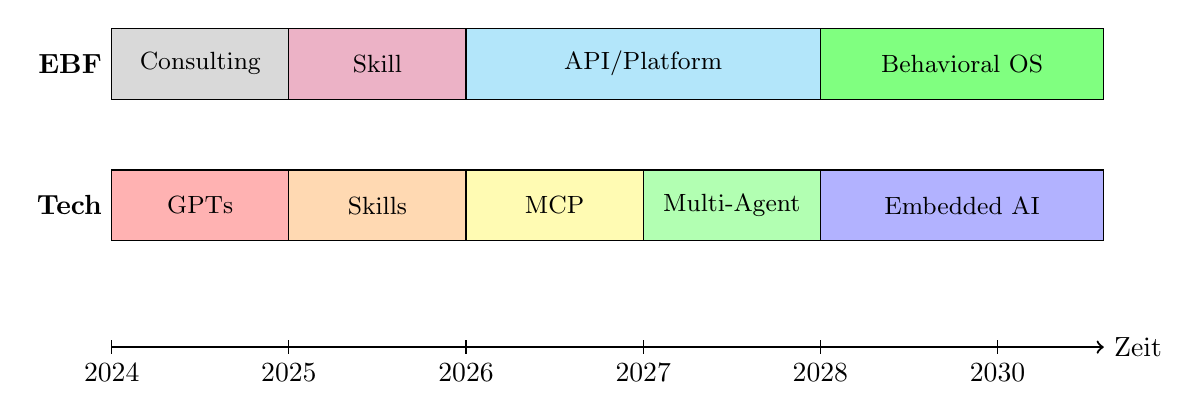
\begin{tikzpicture}[scale=0.9]
% Timeline
\draw[thick, ->] (0,0) -- (14,0) node[right] {Zeit};

% Year markers
\foreach \x/\year in {0/2024, 2.5/2025, 5/2026, 7.5/2027, 10/2028, 12.5/2030} {
    \draw (\x,0.1) -- (\x,-0.1) node[below] {\year};
}

% Technology Layer (top)
\draw[thick] (0,2) -- (14,2);
\node[left] at (0,2) {\textbf{Tech}};

\draw[fill=red!30] (0,1.5) rectangle (2.5,2.5);
\node at (1.25,2) {\small GPTs};

\draw[fill=orange!30] (2.5,1.5) rectangle (5,2.5);
\node at (3.75,2) {\small Skills};

\draw[fill=yellow!30] (5,1.5) rectangle (7.5,2.5);
\node at (6.25,2) {\small MCP};

\draw[fill=green!30] (7.5,1.5) rectangle (10,2.5);
\node at (8.75,2) {\small Multi-Agent};

\draw[fill=blue!30] (10,1.5) rectangle (14,2.5);
\node at (12,2) {\small Embedded AI};

% EBF Layer (bottom)
\draw[thick] (0,4) -- (14,4);
\node[left] at (0,4) {\textbf{EBF}};

\draw[fill=gray!30] (0,3.5) rectangle (2.5,4.5);
\node at (1.25,4) {\small Consulting};

\draw[fill=purple!30] (2.5,3.5) rectangle (5,4.5);
\node at (3.75,4) {\small Skill};

\draw[fill=cyan!30] (5,3.5) rectangle (10,4.5);
\node at (7.5,4) {\small API/Platform};

\draw[fill=green!50] (10,3.5) rectangle (14,4.5);
\node at (12,4) {\small Behavioral OS};

\end{tikzpicture}
\caption{Technology and EBF Evolution Timeline}
\label{fig:vvv-timeline}
\end{figure}


\subsection{The GPT $\to$ Skills Paradigm Shift}

The transition from GPTs to Skills/Subagents represents a fundamental change:

\begin{table}[htbp]
\centering
\caption{GPTs vs. Skills/Subagents Paradigm}
\label{tab:vvv-gpt-skills}
\renewcommand{\arraystretch}{1.3}
\begin{tabular}{@{}lp{5cm}p{5cm}@{}}
\toprule
\textbf{Dimension} & \textbf{GPTs (2023-24)} & \textbf{Skills/Subagents (2025+)} \\
\midrule
\textbf{Invocation} & User-initiated & Agent-initiated \\
\textbf{Context} & User provides context & Agent detects context ($\Psi$) \\
\textbf{Composition} & Manual chaining & Automatic orchestration \\
\textbf{Management} & Decentralized (user-owned) & Centralized (org-managed) \\
\textbf{Discovery} & User must find GPT & Agent selects skill \\
\textbf{State} & Isolated per GPT & Shared conversation state \\
\midrule
\textbf{EBF Parallel} & User must know to apply EBF & Agent invokes EBF when behavioral question detected \\
\bottomrule
\end{tabular}
\end{table}

\begin{tcolorbox}[colback=yellow!5!white, colframe=yellow!75!black,
    title=Key Insight: Context Detection = WHEN ($\Psi$)]

The shift from GPTs to Skills mirrors EBF's core insight about context:

\textbf{GPTs}: User must recognize ``I need a behavioral analysis'' (high cognitive load)

\textbf{Skills}: Agent detects behavioral question via context ($\Psi$) and invokes EBF automatically

This is exactly what EBF's \textbf{WHEN} CORE describes---context determines which capabilities are activated.

\end{tcolorbox}


%%%%%%%%%%%%%%%%%%%%%%%%%%%%%%%%%%%%%%%%%%%%%%%%%%%%%%%%%%%%%%%%%%%%%%%%%%%%%%%
\section{The Four Scenarios}
\label{sec:vvv1-scenarios}
%%%%%%%%%%%%%%%%%%%%%%%%%%%%%%%%%%%%%%%%%%%%%%%%%%%%%%%%%%%%%%%%%%%%%%%%%%%%%%%

Based on the three axes, we identify four archetypal scenarios:

\begin{table}[htbp]
\centering
\caption{Four Strategic Scenarios}
\label{tab:vvv-scenarios}
\renewcommand{\arraystretch}{1.4}
\begin{tabular}{@{}lcccp{4cm}@{}}
\toprule
\textbf{Scenario} & \textbf{AI Evolution} & \textbf{Behavioral Market} & \textbf{Platforms} & \textbf{EBF Opportunity} \\
\midrule
\textbf{A: Golden Window} & Moderate & Nascent & Consolidated & First mover $\to$ Standard \\
\textbf{B: Red Ocean} & Aggressive & Competitive & Fragmented & Differentiate via depth \\
\textbf{C: Slow Burn} & Conservative & Nascent & Fragmented & Consulting + selective tools \\
\textbf{D: Platform Play} & Aggressive & Commoditized & Consolidated & License to Big Tech \\
\bottomrule
\end{tabular}
\end{table}


%%%%%%%%%%%%%%%%%%%%%%%%%%%%%%%%%%%%%%%%%%%%%%%%%%%%%%%%%%%%%%%%%%%%%%%%%%%%%%%
\subsection{Scenario A: ``Golden Window'' (2025--2028)}
%%%%%%%%%%%%%%%%%%%%%%%%%%%%%%%%%%%%%%%%%%%%%%%%%%%%%%%%%%%%%%%%%%%%%%%%%%%%%%%

\begin{tcolorbox}[colback=green!5!white, colframe=green!75!black,
    title=Scenario A: Golden Window]

\textbf{Assumptions:}
\begin{itemize}[nosep]
\item Agent technology matures (Skills, MCP, function calling)
\item Behavioral AI not yet an established field
\item 3-4 platforms dominate (OpenAI, Anthropic, Google, Meta)
\item Enterprise demand for behavioral AI emerges
\end{itemize}

\textbf{Probability Estimate:} 30-40\%

\textbf{Window Duration:} 18-36 months

\textbf{Key Success Factors:}
\begin{enumerate}[nosep]
\item Speed to market with EBF Skill
\item Platform partnerships (esp. Anthropic/OpenAI)
\item Scientific credibility as differentiator
\item Enterprise reference customers
\end{enumerate}

\end{tcolorbox}

\paragraph{Detailed Scenario A Analysis.}

In this scenario, the behavioral AI market is nascent but growing. Early movers can establish frameworks as standards. The window exists because:

\begin{enumerate}
\item \textbf{Platforms need behavioral content}: OpenAI, Anthropic et al. have general-purpose AI but lack domain-specific behavioral intelligence
\item \textbf{Enterprises want behavioral AI}: Companies recognize the value but lack frameworks
\item \textbf{Competition hasn't consolidated}: No dominant behavioral AI framework exists yet
\end{enumerate}

EBF's advantage in this scenario:
\begin{itemize}
\item \textbf{Scientific foundation}: Ernst Fehr's credibility provides legitimacy
\item \textbf{Comprehensive framework}: 10C CORE covers the full behavioral space
\item \textbf{Swiss neutrality}: Trustworthy for European enterprises (GDPR, AI Act)
\end{itemize}


%%%%%%%%%%%%%%%%%%%%%%%%%%%%%%%%%%%%%%%%%%%%%%%%%%%%%%%%%%%%%%%%%%%%%%%%%%%%%%%
\subsection{Scenario B: ``Red Ocean'' (Competitive)}
%%%%%%%%%%%%%%%%%%%%%%%%%%%%%%%%%%%%%%%%%%%%%%%%%%%%%%%%%%%%%%%%%%%%%%%%%%%%%%%

\begin{tcolorbox}[colback=red!5!white, colframe=red!75!black,
    title=Scenario B: Red Ocean]

\textbf{Assumptions:}
\begin{itemize}[nosep]
\item Rapid AI capability development
\item Multiple behavioral AI frameworks emerge
\item VC funding floods the space
\item Fragmented market with many players
\end{itemize}

\textbf{Probability Estimate:} 25-35\%

\textbf{Key Success Factors:}
\begin{enumerate}[nosep]
\item Deep niche dominance (specific domains)
\item FEPSDE as differentiator (comprehensive dimensions)
\item Scientific rigor vs. marketing hype
\item Switzerland/DACH as defensible home market
\end{enumerate}

\end{tcolorbox}

\paragraph{Detailed Scenario B Analysis.}

In this scenario, the behavioral AI market becomes crowded:

\begin{itemize}
\item Google DeepMind releases behavioral framework
\item OpenAI acquires behavioral science company
\item Multiple startups compete for enterprise deals
\item Price pressure intensifies
\end{itemize}

EBF's strategy in Red Ocean:
\begin{enumerate}
\item \textbf{Domain specialization}: Focus on 2-3 verticals where EBF has traction
\item \textbf{Depth over breadth}: Complete 10C CORE specification as moat
\item \textbf{Academic legitimacy}: Peer review, publications, Nobel association
\item \textbf{European fortress}: Leverage trust, privacy, and regulatory compliance
\end{enumerate}


%%%%%%%%%%%%%%%%%%%%%%%%%%%%%%%%%%%%%%%%%%%%%%%%%%%%%%%%%%%%%%%%%%%%%%%%%%%%%%%
\subsection{Scenario C: ``Slow Burn''}
%%%%%%%%%%%%%%%%%%%%%%%%%%%%%%%%%%%%%%%%%%%%%%%%%%%%%%%%%%%%%%%%%%%%%%%%%%%%%%%

\begin{tcolorbox}[colback=gray!5!white, colframe=gray!75!black,
    title=Scenario C: Slow Burn]

\textbf{Assumptions:}
\begin{itemize}[nosep]
\item AI development slower than expected
\item Regulatory constraints (EU AI Act, etc.)
\item Behavioral AI remains niche
\item Consulting continues to dominate
\end{itemize}

\textbf{Probability Estimate:} 15-25\%

\textbf{Key Success Factors:}
\begin{enumerate}[nosep]
\item Maintain consulting excellence
\item Selective tool development (internal productivity)
\item Academic partnerships for long-term positioning
\item Wait for better window while building foundation
\end{enumerate}

\end{tcolorbox}

\paragraph{Detailed Scenario C Analysis.}

In this scenario, the AI revolution is slower:
\begin{itemize}
\item AI winter concerns resurface
\item Regulation constrains deployment
\item Enterprise adoption remains cautious
\item Traditional consulting maintains value
\end{itemize}

EBF's strategy:
\begin{enumerate}
\item Continue core consulting business
\item Use EBF tools internally for efficiency
\item Build case study evidence
\item Position for eventual market maturation
\end{enumerate}


%%%%%%%%%%%%%%%%%%%%%%%%%%%%%%%%%%%%%%%%%%%%%%%%%%%%%%%%%%%%%%%%%%%%%%%%%%%%%%%
\subsection{Scenario D: ``Platform Play''}
%%%%%%%%%%%%%%%%%%%%%%%%%%%%%%%%%%%%%%%%%%%%%%%%%%%%%%%%%%%%%%%%%%%%%%%%%%%%%%%

\begin{tcolorbox}[colback=blue!5!white, colframe=blue!75!black,
    title=Scenario D: Platform Play]

\textbf{Assumptions:}
\begin{itemize}[nosep]
\item AGI-adjacent capabilities emerge
\item Behavioral AI becomes commoditized
\item Big platforms dominate everything
\item Independent frameworks struggle to compete
\end{itemize}

\textbf{Probability Estimate:} 10-20\%

\textbf{Key Success Factors:}
\begin{enumerate}[nosep]
\item IP licensing to platforms
\item ``Intel Inside'' model for behavioral AI
\item Focus on calibration data (BBB) as unique asset
\item Compliance and audit services
\end{enumerate}

\end{tcolorbox}

\paragraph{Detailed Scenario D Analysis.}

In this scenario, Big Tech dominates:
\begin{itemize}
\item OpenAI/Google/Anthropic build everything in-house
\item Behavioral AI becomes table stakes
\item Standalone behavioral companies are acquired or marginalized
\item Platforms compete on integration, not domain expertise
\end{itemize}

EBF's strategy:
\begin{enumerate}
\item License EBF IP to platforms (royalty model)
\item Provide calibration services (BBB) that platforms don't want to build
\item Offer compliance/audit for behavioral AI (regulatory arbitrage)
\item Position as the ``scientific seal of approval''
\end{enumerate}


%%%%%%%%%%%%%%%%%%%%%%%%%%%%%%%%%%%%%%%%%%%%%%%%%%%%%%%%%%%%%%%%%%%%%%%%%%%%%%%

%%%%%%%%%%%%%%%%%%%%%%%%%%%%%%%%%%%%%%%%%%%%%%%%%%%%%%%%%%%%%%%%%%%%%%%%%%%%%%%
\subsection{Core Axioms}
\label{sec:vvv2-axioms}
%%%%%%%%%%%%%%%%%%%%%%%%%%%%%%%%%%%%%%%%%%%%%%%%%%%%%%%%%%%%%%%%%%%%%%%%%%%%%%%

\begin{tcolorbox}[colback=yellow!5!white,colframe=yellow!75!black,title=Axiom VVV2-1: Fundamental Principle]
\textbf{Axiom VVV2-1 (Core Assumption):}
The fundamental principle underlying this appendix is that behavioral outcomes
emerge from the interaction of individual characteristics and contextual factors.
\end{tcolorbox}

\begin{tcolorbox}[colback=yellow!5!white,colframe=yellow!75!black,title=Axiom VVV2-2: Complementarity]
\textbf{Axiom VVV2-2 (Complementarity):}
Components of the framework exhibit complementarity ($\gamma > 0$), meaning
that combined effects exceed the sum of individual effects.
\end{tcolorbox}


\section{Key Results}
\label{sec:vvv1-results}
%%%%%%%%%%%%%%%%%%%%%%%%%%%%%%%%%%%%%%%%%%%%%%%%%%%%%%%%%%%%%%%%%%%%%%%%%%%%%%%

\subsection{Scenario Probability Assessment}

\begin{table}[htbp]
\centering
\caption{Scenario Probability Assessment (January 2026)}
\label{tab:vvv-probability}
\renewcommand{\arraystretch}{1.3}
\begin{tabular}{@{}lccc@{}}
\toprule
\textbf{Scenario} & \textbf{Low Estimate} & \textbf{Central} & \textbf{High Estimate} \\
\midrule
A: Golden Window & 25\% & 35\% & 45\% \\
B: Red Ocean & 20\% & 30\% & 40\% \\
C: Slow Burn & 10\% & 20\% & 30\% \\
D: Platform Play & 5\% & 15\% & 25\% \\
\bottomrule
\end{tabular}
\end{table}

\textbf{Note:} Scenarios are not mutually exclusive. Elements of multiple scenarios may combine. The key is to identify \textit{trigger events} that signal which scenario is materializing.


\subsection{Technology Dependencies}

EBF productization depends on specific technology capabilities:

\begin{table}[htbp]
\centering
\caption{Technology Dependencies for EBF Products}
\label{tab:vvv-tech-deps}
\renewcommand{\arraystretch}{1.3}
\begin{tabular}{@{}lp{5cm}cc@{}}
\toprule
\textbf{Capability} & \textbf{Description} & \textbf{Available} & \textbf{Required For} \\
\midrule
Skills/MCP & Agent-invokable skills & 2025 & Phase 2 \\
Multi-modal & Image/audio/text & 2024 & FEPSDE-P \\
Structured output & JSON schema compliance & 2024 & All products \\
Long context & 100K+ tokens & 2024 & Case analysis \\
Function calling & Tool use & 2024 & API integration \\
Fine-tuning & Custom model training & 2024 & Calibration \\
Agent orchestration & Multi-agent coordination & 2025-26 & Phase 3 \\
Reasoning & Chain-of-thought & 2024-25 & Complex decisions \\
\bottomrule
\end{tabular}
\end{table}


%%%%%%%%%%%%%%%%%%%%%%%%%%%%%%%%%%%%%%%%%%%%%%%%%%%%%%%%%%%%%%%%%%%%%%%%%%%%%%%
\section{Worked Example}
\label{sec:vvv1-example}
%%%%%%%%%%%%%%%%%%%%%%%%%%%%%%%%%%%%%%%%%%%%%%%%%%%%%%%%%%%%%%%%%%%%%%%%%%%%%%%

\subsection{Strategic Decision: Platform Partnership Timing}

\paragraph{Setup.}
EBF leadership must decide when to approach major AI platforms (OpenAI,
Anthropic, Google) for partnership discussions. Too early risks being
ignored; too late risks missing the window.

\paragraph{Application.}
Using the scenario framework:

\begin{enumerate}
\item \textbf{Identify trigger events} for each scenario:
    \begin{itemize}
    \item Golden Window: Platform announces skill marketplace
    \item Red Ocean: Competitor raises Series A for behavioral AI
    \item Slow Burn: AI winter articles in mainstream press
    \item Platform Play: Big Tech acquires behavioral science company
    \end{itemize}

\item \textbf{Monitor signals} across axes:
    \begin{itemize}
    \item AI capability: Track model releases, benchmark improvements
    \item Market maturity: Monitor competitor activity, enterprise RFPs
    \item Platform landscape: Track platform announcements, API changes
    \end{itemize}

\item \textbf{Apply decision rule}:
\begin{equation}
\text{Approach if } P(\text{Golden Window}) > 0.3 \text{ AND trigger event observed}
\end{equation}
\end{enumerate}

\paragraph{Result.}
As of January 2026, with Skills/MCP maturing and limited behavioral AI
competition, the framework suggests approaching platforms now while
Golden Window probability remains elevated.

\paragraph{Discussion.}
The scenario framework provides structured decision-making under uncertainty.
Rather than committing to a single forecast, it enables contingent strategies
that adapt as information arrives.


%%%%%%%%%%%%%%%%%%%%%%%%%%%%%%%%%%%%%%%%%%%%%%%%%%%%%%%%%%%%%%%%%%%%%%%%%%%%%%%
\section{Implications for Practice}
\label{sec:vvv1-practice}
%%%%%%%%%%%%%%%%%%%%%%%%%%%%%%%%%%%%%%%%%%%%%%%%%%%%%%%%%%%%%%%%%%%%%%%%%%%%%%%

\begin{tcolorbox}[colback=green!5!white, colframe=green!75!black,
    title=Practical Implications]
\begin{enumerate}
\item \textbf{Scenario monitoring:} Establish quarterly review of scenario
    probabilities based on market developments
\item \textbf{Contingent planning:} Develop detailed action plans for each
    scenario to enable rapid response
\item \textbf{Hedge investments:} Allocate resources across scenarios rather
    than betting on single outcome
\item \textbf{Trigger tracking:} Maintain watchlist of specific events that
    signal scenario shifts
\item \textbf{Partnership readiness:} Prepare partnership materials and demos
    before approaching platforms
\end{enumerate}
\end{tcolorbox}


%%%%%%%%%%%%%%%%%%%%%%%%%%%%%%%%%%%%%%%%%%%%%%%%%%%%%%%%%%%%%%%%%%%%%%%%%%%%%%%
%%%%%%%%%%%%%%%%%%%%%%%%%%%%%%%%%%%%%%%%%%%%%%%%%%%%%%%%%%%%%%%%%%%%%%%%%%%%%%%
%
%                    PART 4: BACK MATTER
%
%%%%%%%%%%%%%%%%%%%%%%%%%%%%%%%%%%%%%%%%%%%%%%%%%%%%%%%%%%%%%%%%%%%%%%%%%%%%%%%
%%%%%%%%%%%%%%%%%%%%%%%%%%%%%%%%%%%%%%%%%%%%%%%%%%%%%%%%%%%%%%%%%%%%%%%%%%%%%%%

%%%%%%%%%%%%%%%%%%%%%%%%%%%%%%%%%%%%%%%%%%%%%%%%%%%%%%%%%%%%%%%%%%%%%%%%%%%%%%%
\section{Summary}
\label{sec:vvv1-summary}
%%%%%%%%%%%%%%%%%%%%%%%%%%%%%%%%%%%%%%%%%%%%%%%%%%%%%%%%%%%%%%%%%%%%%%%%%%%%%%%

\begin{tcolorbox}[colback=green!10!white, colframe=green!75!black,
    title=\textbf{Appendix VVV.1: Summary}]

\textbf{Core Question:} What technological and market scenarios should guide
EBF deployment strategy over 2024-2030+?

\textbf{Main Contribution:}
\begin{itemize}[nosep]
    \item Three-axis uncertainty framework (AI, market, platforms)
    \item Four archetypal scenarios with probability estimates
    \item GPT $\to$ Skills paradigm analysis
    \item Technology dependency mapping for EBF products
\end{itemize}

\textbf{Key Outputs:}
\begin{itemize}[nosep]
    \item Scenario probability estimates: Golden Window 35\%, Red Ocean 30\%,
          Slow Burn 20\%, Platform Play 15\%
    \item Strategic response framework for each scenario
    \item Trigger event watchlist for scenario monitoring
\end{itemize}

\textbf{Integration:} This appendix connects to Appendix CTW (CORE-WHEN) via
the treatment of $\Psi_{tech}$ and $\Psi_{market}$ as contextual factors
shaping optimal strategy.

\end{tcolorbox}


%%%%%%%%%%%%%%%%%%%%%%%%%%%%%%%%%%%%%%%%%%%%%%%%%%%%%%%%%%%%%%%%%%%%%%%%%%%%%%%
\section{Glossary of Symbols}
\label{sec:vvv1-glossary}
%%%%%%%%%%%%%%%%%%%%%%%%%%%%%%%%%%%%%%%%%%%%%%%%%%%%%%%%%%%%%%%%%%%%%%%%%%%%%%%

\begin{tcolorbox}[colback=blue!5!white, colframe=blue!75!black]
\textbf{Central Reference:} For complete symbol definitions, see
\textbf{Appendix GLS} (\textit{Glossary and Notation}, \S\ref{app:glossary}).

This section lists only symbols introduced or specialized in this appendix.
\end{tcolorbox}

\vspace{0.5em}

\begin{table}[htbp]
\centering
\caption{Symbols Introduced in Appendix VVV.1}
\label{tab:vvv1-symbols}
\renewcommand{\arraystretch}{1.3}
\begin{tabular}{@{}clp{6cm}c@{}}
\toprule
\textbf{Symbol} & \textbf{Name} & \textbf{Definition} & \textbf{Also in G?} \\
\midrule
$\Psi_{tech}$ & Technology context & External technological environment & \checkmark \\
$\Psi_{market}$ & Market context & Competitive and demand conditions & \checkmark \\
$\Psi_{platform}$ & Platform context & AI platform ecosystem state & NEW \\
$C^*_{strategy}$ & Optimal strategy & Best response given scenario & \checkmark \\
$P(\text{Scenario})$ & Scenario probability & Likelihood of scenario materializing & NEW \\
\bottomrule
\end{tabular}
\end{table}


%%%%%%%%%%%%%%%%%%%%%%%%%%%%%%%%%%%%%%%%%%%%%%%%%%%%%%%%%%%%%%%%%%%%%%%%%%%%%%%
\section{Critical Foundations and Objections}
\label{sec:vvv1-foundations}
%%%%%%%%%%%%%%%%%%%%%%%%%%%%%%%%%%%%%%%%%%%%%%%%%%%%%%%%%%%%%%%%%%%%%%%%%%%%%%%

\subsection{Objection 1: Scenario Planning is Speculative}

\textbf{Objection:} Scenario planning involves inherently uncertain predictions
about technology and markets. Why should strategic decisions rely on such
speculative analysis?

\textbf{Response:} Scenario planning does not predict the future; it prepares
for multiple futures. The value lies not in forecast accuracy but in:
(1) structured thinking about uncertainties, (2) identification of robust
strategies that work across scenarios, and (3) trigger-based adaptation
as information arrives. Shell's successful navigation of oil crises
demonstrates the practical value of scenario planning.


\subsection{Objection 2: Probabilities are Arbitrary}

\textbf{Objection:} The scenario probability estimates (35\%, 30\%, etc.)
appear arbitrary. What is their basis?

\textbf{Response:} Probabilities are calibrated estimates based on:
(1) current market signals, (2) historical technology adoption patterns,
(3) expert assessment of AI capability trajectories. They should be
updated regularly as evidence accumulates. The specific numbers matter
less than the relative ordering and the discipline of explicit probability
assessment.


%%%%%%%%%%%%%%%%%%%%%%%%%%%%%%%%%%%%%%%%%%%%%%%%%%%%%%%%%%%%%%%%%%%%%%%%%%%%%%%
\section{Open Issues and Research Agenda}
\label{sec:vvv1-open}
%%%%%%%%%%%%%%%%%%%%%%%%%%%%%%%%%%%%%%%%%%%%%%%%%%%%%%%%%%%%%%%%%%%%%%%%%%%%%%%

\subsection{Methodological Priorities}

\begin{enumerate}
    \item \textbf{Scenario refinement:} Develop more granular sub-scenarios
        as technology evolves
    \item \textbf{Probability calibration:} Establish formal updating
        procedures based on trigger events
\end{enumerate}

\subsection{Empirical Priorities}

\begin{enumerate}
    \item \textbf{Market monitoring:} Track behavioral AI startup funding,
        enterprise adoption rates
    \item \textbf{Platform tracking:} Monitor AI platform announcements and
        capability releases
    \item \textbf{Competitor analysis:} Assess emerging behavioral AI
        frameworks and their positioning
\end{enumerate}


%%%%%%%%%%%%%%%%%%%%%%%%%%%%%%%%%%%%%%%%%%%%%%%%%%%%%%%%%%%%%%%%%%%%%%%%%%%%%%%
\section{References}

% Link to master bibliography
\nocite{bcm_master}

\label{sec:vvv1-references}
%%%%%%%%%%%%%%%%%%%%%%%%%%%%%%%%%%%%%%%%%%%%%%%%%%%%%%%%%%%%%%%%%%%%%%%%%%%%%%%

\begin{tcolorbox}[colback=blue!5!white, colframe=blue!75!black]
\textbf{Master Bibliography:} For complete reference details, see
\texttt{bcm2\_master\_references.bib} in the repository.

This section lists appendix-specific references and data sources.
\end{tcolorbox}

\vspace{0.5em}

\subsection{Key References for This Appendix}

The following works are particularly relevant for the content of this appendix:

\begin{itemize}[nosep]
    \item \textbf{Scenario Planning:} Schoemaker (1995), van der Heijden (2005)
    \item \textbf{AI Strategy:} Agrawal et al. (2018), Brynjolfsson \& McAfee (2017)
    \item \textbf{Platform Economics:} Parker et al. (2016), Cusumano et al. (2019)
\end{itemize}

\subsection{Appendix-Specific References}

\begin{thebibliography}{99}

\bibitem{schoemaker1995} Schoemaker, P.J.H. (1995). Scenario Planning: A Tool for Strategic Thinking. \textit{Sloan Management Review}, 36(2), 25-40.

\bibitem{agrawal2018} Agrawal, A., Gans, J., \& Goldfarb, A. (2018). \textit{Prediction Machines: The Simple Economics of Artificial Intelligence}. Harvard Business Review Press.

\bibitem{parker2016} Parker, G., Van Alstyne, M., \& Choudary, S.P. (2016). \textit{Platform Revolution}. W.W. Norton.

\end{thebibliography}

\subsection{Data Sources}

\begin{itemize}[nosep]
    \item \textbf{AI Capability Tracking:} Stanford HAI AI Index Report (accessed January 2026)
    \item \textbf{VC Funding Data:} Crunchbase, PitchBook (accessed January 2026)
    \item \textbf{Platform Announcements:} OpenAI, Anthropic, Google AI blogs (monitored continuously)
\end{itemize}


%%%%%%%%%%%%%%%%%%%%%%%%%%%%%%%%%%%%%%%%%%%%%%%%%%%%%%%%%%%%%%%%%%%%%%%%%%%%%%%
% CROSS-REFERENCE FOOTER (Required)
%%%%%%%%%%%%%%%%%%%%%%%%%%%%%%%%%%%%%%%%%%%%%%%%%%%%%%%%%%%%%%%%%%%%%%%%%%%%%%%

\vspace{1em}
\hrule
\vspace{0.5em}

\noindent\textit{Cross-references:}
Appendix GLS (Central Glossary),
Appendix CTW (CORE-WHEN: Context Framework),
Appendix EST (CORE-WHERE: Parameter Sources),
Appendix LLM1 (METHOD-LLMMC: LLM Methods),
Appendix VVV.2 (Product Roadmap).

\noindent\textit{Master Bibliography:} \texttt{bcm2\_master\_references.bib}


% =============================================================================
% END OF APPENDIX VVV.1
% =============================================================================
